L'Hypertext Transfer Protocol ( HTTP) est un protocole Client/Serveur. Il fonctionne sur tous types de connexions. Il est basé sur le proctocole TCP. 
Le protocole HTTP  basé sur la couche application tandis que le TCP est basé sur la couche de transport.
\begin{figure}[h]
    \centering
    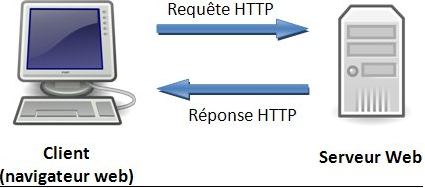
\includegraphics[width=100mm, height=40mm]{images/HTTP2.png}
    \caption{Schéma explicatif HTTP simplifié}
    \label{img:mesh11}
\end{figure}
\begin{figure}[h]
    \centering
    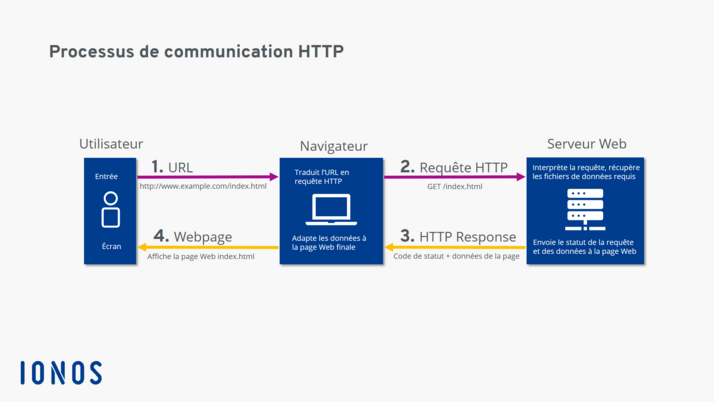
\includegraphics[width=150mm, height=80mm]{images/HTTP1.png}
    \caption{Schéma explicatif HTTP détaillé}
    \label{img:mesh12}
\end{figure}
\newpage